% CS4246/5446 AY2627 S1 -- Final Report
% Single-spaced, single-column, 12pt, 1in margins. Figures are produced by
% make_figures.py in this directory from saved run artifacts.
\documentclass[12pt,a4paper]{article}

\usepackage[margin=1in]{geometry}
\usepackage[T1]{fontenc}
\usepackage{mathptmx}
% Times digits and letters in math; the symbol font stays Computer Modern because the
% Times-matched symbol font needs rsfs, which is not installed here.
\DeclareSymbolFont{symbols}{OMS}{cmsy}{m}{n}
\renewcommand{\ttdefault}{lmtt}
\usepackage{amsmath}
\usepackage{enumitem}
\usepackage{booktabs}
\usepackage{array}
\usepackage{tabularx}
\usepackage{graphicx}
\usepackage[font=normalsize,labelfont=bf,skip=4pt]{caption}
\usepackage{float}
\usepackage{xcolor}
\usepackage{titlesec}
\usepackage{microtype}
\usepackage[hidelinks]{hyperref}

\titleformat{\section}{\normalfont\large\bfseries}{\thesection}{0.6em}{}
\titleformat{\subsection}{\normalfont\normalsize\bfseries}{\thesubsection}{0.6em}{}
\titlespacing{\section}{0pt}{10pt plus 2pt minus 2pt}{4pt}
\titlespacing{\subsection}{0pt}{8pt plus 2pt minus 2pt}{3pt}
\setlist{topsep=2pt,itemsep=1pt,parsep=0pt,leftmargin=*}
\setlength{\parskip}{4pt}
\setlength{\parindent}{0pt}
\setlength{\textfloatsep}{10pt plus 2pt minus 2pt}
\setlength{\floatsep}{8pt plus 2pt minus 2pt}
\setlength{\intextsep}{8pt plus 2pt minus 2pt}
\renewcommand{\topfraction}{0.85}
\renewcommand{\bottomfraction}{0.6}
\renewcommand{\textfraction}{0.12}
\renewcommand{\floatpagefraction}{0.75}
\renewcommand{\arraystretch}{1.1}

% Unit used in text and in math; in math it is set upright, not as a product of variables.
\DeclareRobustCommand{\bps}{\ifmmode\,\text{bps}\else\,bps\fi}
\newcommand{\todo}[1]{\fcolorbox{red!70!black}{red!6}{\parbox{\dimexpr\linewidth-2\fboxsep-2\fboxrule}{\textbf{TODO (team):} #1}}}

\begin{document}
\pagenumbering{Alph}

% ------------------------------------------------------------------ title page
\begin{titlepage}
\centering
\vspace*{1.2cm}
{\large National University of Singapore \\ School of Computing \par}
\vspace{0.4cm}
{\large CS4246/5446 --- Reinforcement Learning and Sequential Decision Making \\
Semester 1, AY2026/27 \par}
\vspace{1.4cm}
{\LARGE\bfseries Final Report \par}
\vspace{0.5cm}
{\Large Learning When \emph{Not} to Trade: Reinforcement Learning for \\[2pt]
Cross-Venue Latency Arbitrage After Transaction Costs \par}
\vspace{1.6cm}
{\large Group X \quad\textbar\quad Application Project \par}
\vspace{1.1cm}

\begin{tabular}{@{}lll@{}}
\toprule
\textbf{Name} & \textbf{Matriculation No.} & \textbf{Email} \\
\midrule
Kerk Tai Heng      & A0XXXXXXX & e1137106@u.nus.edu \\
$\langle$Member 2$\rangle$ & A0XXXXXXX & eXXXXXXX@u.nus.edu \\
$\langle$Member 3$\rangle$ & A0XXXXXXX & eXXXXXXX@u.nus.edu \\
$\langle$Member 4$\rangle$ & A0XXXXXXX & eXXXXXXX@u.nus.edu \\
$\langle$Member 5$\rangle$ & A0XXXXXXX & eXXXXXXX@u.nus.edu \\
$\langle$Member 6$\rangle$ & A0XXXXXXX & eXXXXXXX@u.nus.edu \\
\bottomrule
\end{tabular}

\vspace{0.8cm}
{\normalsize\textit{AI-use disclosure: AI coding agents implemented substantial parts of the
software and drafted this report under the team's direction. The full statement follows the
conclusion.}\par}

\vfill
{\normalsize 5 October 2026 \par}
\end{titlepage}

\pagenumbering{arabic}
\setcounter{page}{1}

% ------------------------------------------------------------------ abstract
\phantomsection\label{bodystart}
\begin{center}{\large\bfseries Abstract}\end{center}
\vspace{-4pt}
We asked whether a reinforcement learning agent can trade Bitcoin perpetual futures
between Binance and Hyperliquid only when the price gap between the two venues is large
enough to pay for fees, spread and execution delay, and stay flat otherwise. We prepared
30 days of recorded order books (3 September to 2 October 2026, UTC) into 8,245 causally
aligned five-minute replay episodes and built a Gymnasium environment that fills orders
150\,ms after the decision against the recorded Hyperliquid book and charges a taker fee on
each fill. Two PPO designs were trained and selected on validation days only. The first, a
four-action policy trained for one million steps on three seeds plus a higher-entropy retry,
cut its share of entry actions below 1\% within about 230,000 steps; the selected policy made
zero trades on validation and on the four held-out test days. A fixed rule that enters when
the gap reaches 10 basis points (bps; 1\bps{} is 0.01\%), run as a control in the same
environment, made 16 test trades for a net \$1.19 with a taker fee of 3.5\bps{} on each fill.
At 4.5\bps{} per fill, the rate we used later, the same selection procedure would have
picked a threshold that never trades. The second design, a skip-or-enter decision at screened
candidate gaps with a supervised warm start, also ended with zero validation trades for all
three PPO seeds. We report properties of the problem that are consistent with the failure,
without testing which of them caused it: gaps of 7\bps{} or more, roughly one round-trip
cost, occurred in under 0.1\% of validation and test seconds (0.084\% and 0.097\%); staying
flat returns exactly zero while early trading loses money; and 99.7\% of the training seconds
with a gap of 7\bps{} or more fell in a six-day period when the two venues' prices were offset
and did not converge. A weaker offset of the same kind recurred on validation (daily median
$-2.8$\bps{} on 25 September). A zero-trade policy is abstention, and we report it as a failure
to learn the intended behaviour.

% ------------------------------------------------------------------ 1
\section{Introduction}\label{sec:intro}

Bitcoin perpetual futures (futures contracts with no expiry date) trade on many venues at
the same time, and a price move does not reach every venue's order book at the same moment.
A trader who sees a move first on one venue can buy or sell on a venue whose quotes have not
yet adjusted, then exit when the two prices converge. This is latency arbitrage. Budish,
Cramton and Shim~\cite{budish} describe the same mechanism in equity markets, where fast
traders profit by trading against quotes that have not yet caught up with a price change
elsewhere.

An order book lists resting buy orders (bids) and sell orders (asks) at each price level.
The best bid and the best ask form the top of the book, the spread is the best ask minus the
best bid, and depth is the size available at the displayed levels. The mid price is the
average of the best bid and the best ask. We measure the gap as the Binance mid minus the
Hyperliquid mid, divided by the Hyperliquid mid, in basis points (bps; 1\bps{} is 0.01\%).
Across the 2,473,500 one-second decision rows we kept, the median absolute gap was
1.29\bps.

A visible gap is not a profit. An order that executes immediately against resting orders is
a taker order: it buys at the ask and sells at the bid, so relative to the mid it pays half
the spread on each fill and one full spread over a round trip (entry and exit). Each fill
also pays a taker fee and can suffer slippage, an execution price worse than the quoted one.
Below, ``per side'' means per fill. With our base assumptions of a 3.5\bps{} fee and
0.1\bps{} slippage per side, and a median Hyperliquid spread of about 0.12\bps, a round trip
costs $2\times3.5 + 2\times0.1 + 0.12 \approx 7.3$\bps; at 4.5\bps{} per side, the fee in our
second attempt, it costs about 9.3\bps. On the validation and test days, fewer than 0.1\% of
decision seconds had an absolute gap of 7\bps{} or more. A profitable policy has to trade
only on the few gaps larger than this cost. The internal feasibility study that motivated the
project reported similar magnitudes: a median gap of about 1\bps{} against a round-trip cost
of about 7\bps~\cite{report}.

Our research question was whether proximal policy optimisation (PPO)~\cite{ppo} can learn
this selective behaviour from recorded order books with all costs in the reward, and beat a
fixed threshold rule under identical costs on later, unseen days. Reinforcement learning has
been applied to related microstructure problems such as optimal order
execution~\cite{nevmyvaka}. Here, profitable entries are rare and staying flat returns exactly
zero. The proposal rated ``RL training is unstable or learns only to abstain'' as a medium
risk, and abstention is what happened. Two PPO designs, with seven trained PPO policies
between them, ended with zero validation trades, and the selected policy of the first design
also made zero trades on the held-out test, while a 10\bps{} threshold control made a small
profit there.

The project produced a quality-checked, causally aligned replay dataset with a SHA-256 hash
for every episode; a replay environment with delayed fills against the recorded book, fees on
both sides, and freshness and risk checks, covered by 41 environment tests and 20 evaluation
tests, all passing (the tracked suite has 168 tests); two pre-declared PPO experiments with
validation-only selection and a single test evaluation; and an analysis of the failure based
on the training logs and the data (Section~\ref{sec:why}). Section~\ref{sec:conclusion} lists
the changes we would make next.

% ------------------------------------------------------------------ 2
\section{Data}\label{sec:data}

\subsection{Source and research range}
The team recorded both venues' public order-book streams into one ClickHouse table. Each row
is one book snapshot with the exchange timestamp, the local receive timestamp, and bid and
ask price and size arrays. Binance rows come from the \texttt{btcusdt@depth20@100ms} stream
and always have 20 levels per side. Hyperliquid rows come from its \texttt{l2Book} stream and
always have 5 levels per side; the proposal had assumed 10 levels for both. The data are
public market feeds and contain no personal information. An inventory taken at 16:30 UTC on
3 October 2026 counted 32,888,724 rows (27,464,104 Binance and 5,424,620 Hyperliquid).
Capture began on 27 August, but an outage left 30 August almost empty, 31 August and
1 September missing, and 2 September partial. Before any modelling we fixed the research
range to the 30 complete days from 3 September to 2 October, which hold 28,917,283 raw rows
(24,146,574 Binance and 4,770,709 Hyperliquid). The split is chronological: 22 days for
training, 4 for validation and 4 for testing (Table~\ref{tab:data}). The day of 3 October
(780,739 Binance and 158,589 Hyperliquid rows) was prepared later as a separate holdout.

\begin{table}[!htbp]
\centering
\caption{Splits and gap statistics on prepared one-second decision rows. Gap is
$10^4\times(\text{Binance mid} - \text{Hyperliquid mid})/\text{Hyperliquid mid}$.
``Dropped'' counts five-minute windows rejected by the quality filter.}
\label{tab:data}
\begin{tabular}{@{}llrrrrr@{}}
\toprule
 & & Windows & & \multicolumn{2}{c}{$|$gap$|$ (bps)} & Seconds with \\
\cmidrule(lr){5-6}
Split & Dates (2026) & (dropped) & Decisions & Median & p99 & $|$gap$|\geq 7$\bps{} \\
\midrule
Train      & 3--24 Sep   & 5,984 (352) & 1,795,200 & 1.34 & 12.57 & 18.04\% \\
Validation & 25--28 Sep  & 1,121 (31)  &   336,300 & 1.30 &  5.20 & 0.084\% \\
Test       & 29 Sep--2 Oct & 1,140 (12) &  342,000 & 1.04 &  4.86 & 0.097\% \\
Fresh day  & 3 Oct       &   286 (2)   &    85,800 & 0.61 &  2.31 & 0.0047\% \\
\bottomrule
\end{tabular}
\end{table}

\subsection{Causal alignment and quality filtering}\label{sec:align}
Decisions are made on a grid of whole UTC seconds. Each decision second also has two
execution rows, at +150\,ms and +300\,ms, which are used to fill delayed orders, so the
replay has three rows per second. Every grid row takes, for each venue, the latest snapshot
received at or before its timestamp, so no row uses information that arrived later. Each
grid row also records two ages per venue: the receive age, the row's time minus the local
receive time of that snapshot, and the quote age, the row's time minus the snapshot's
exchange timestamp. A grid row was marked invalid if either venue had no earlier snapshot; if
the latest snapshot failed the validity checks (finite positive prices and sizes, strictly
ordered levels, a best bid below the best ask); if the receive age exceeded 2,000\,ms or the
quote age exceeded 3,000\,ms; if a spread exceeded 100\bps; or if the gap exceeded 250\bps.
Episodes are fixed 300-second UTC windows (900 rows and 300 decisions). A window with any
invalid row was dropped whole, so a feed outage never appears inside an episode
(Section~\ref{sec:subset} discusses the bias this creates).

Of 8,640 windows, 8,245 (95.43\%) were kept. Hyperliquid staleness caused almost every
rejection: 3,180 grid rows failed the receive-age rule and 3,065 the quote-age rule on
Hyperliquid, against 176 and 166 on Binance, and no row failed the validity, spread or gap
rules. Hyperliquid had 504 receive gaps longer than 2\,s in the range (the longest 173\,s,
on 26 September); Binance had 9. Feed quality improved late in the period: training days
lost 9 to 21 windows each, while from 27 September onward only 1 to 4 windows per day were
lost. One rejection per day is an artefact of the preparation code. Each day is cached
separately, so the 00:00:00 grid row has no earlier record and the 00:00--00:05 window is
always dropped; this accounts for 30 of the 395 rejections. Appendix~\ref{app:quality}
gives the counts by reason and day.

\subsection{Venue asymmetry}\label{sec:asym}
Over the 30 days, Binance's 100\,ms depth stream delivered 9.32 snapshots per second (the
stream's cap is 10) and Hyperliquid's \texttt{l2Book} stream 1.84. The update rate alone does
not show which venue moves first; Section~\ref{sec:val1} tests whether the gap predicts
Hyperliquid's next move. At decision rows the median Hyperliquid quote age was 623, 627 and
640\,ms on the training, validation and test splits, with a 99th percentile of 1.06 to
1.12\,s. Part of that figure is the receive age, the time since the snapshot arrived, whose
median was about 270\,ms on every split. Receive time minus exchange timestamp had a
median of 335, 339 and 350\,ms and a 99th percentile of 0.60 to 0.65\,s. This difference
mixes network delay with any offset between the exchange clock and the recorder clock, so it
is not a pure latency measurement. The proposal's figure of about 285\,ms came from an
earlier calculation whose definition we could not trace, so we do not compare with it. The
median top-of-book spread was about 0.012\bps{} on Binance and 0.12\bps{} on Hyperliquid.

Because perpetual futures never expire, each venue keeps its contract price near the spot
index price with funding: periodic payments between holders of long and short positions, at
a rate the venue sets. A difference in funding between venues can therefore sustain a price
offset between them. Funding payments, which the proposal planned to include in the reward, are not in the
source table, and the funding rate is set to zero throughout (Section~\ref{sec:funding}).

\subsection{Gap distribution and the 18--23 September offset}\label{sec:basis}
\begin{figure}[!htbp]
\centering
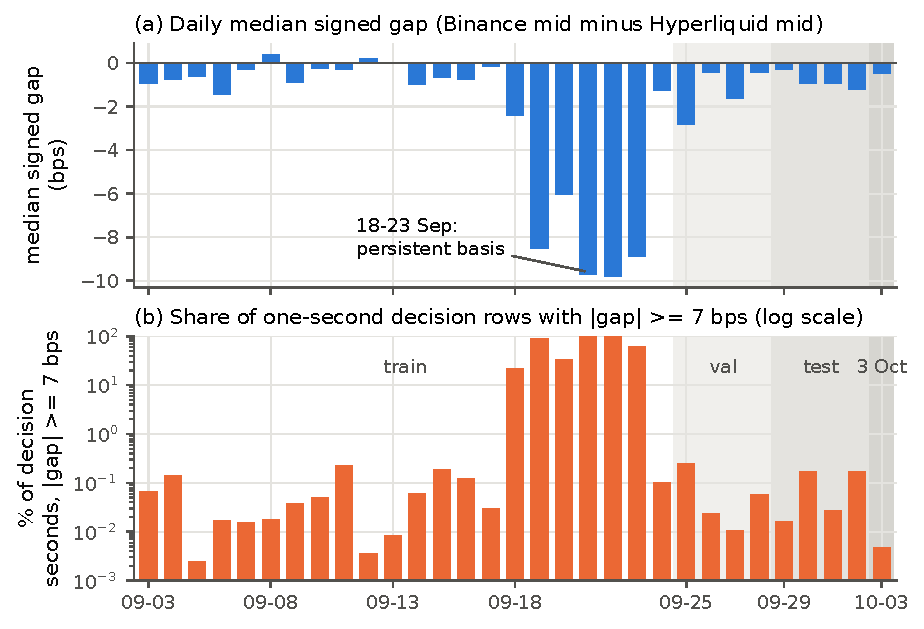
\includegraphics{figures/fig_daily_gap.pdf}
\caption{Daily cross-venue gap on prepared decision rows, 3 September to 3 October 2026.
(a) Median signed gap. (b) Share of decision seconds with an absolute gap of at least
7\bps, roughly one round-trip cost, on a log scale. Shading marks the training (white),
validation, test and fresh-day periods. Six training days carry almost all large gaps.}
\label{fig:gap}
\end{figure}

As a check on the preparation, we recomputed the reference statistics in the team's data
guide~\cite{guide} for 15 September with the guide's own method (last snapshot in each
one-second bucket, inner join of the two venues). We obtained a median absolute gap of
0.940\bps{} against the quoted 0.956, a 99th percentile of 4.36 against 4.30, and 0.218\% of
seconds above 7\bps, equal to the quoted value. Our causal episodes for the same day gave
0.931, 4.27 and 0.185\%.

The training split has far more large gaps than the later splits (Table~\ref{tab:data}): on
training days 18.04\% of decision seconds had an absolute gap of at least 7\bps, against
0.084\% on validation, 0.097\% on test and 0.0047\% (4 seconds) on 3 October.
Figure~\ref{fig:gap} shows when they occurred. From 18 to 23 September the Binance mid sat
below the Hyperliquid mid for whole days, with daily median signed gaps of $-2.4$, $-8.5$,
$-6.1$, $-9.7$, $-9.8$ and $-8.9$\bps. These six days hold 322,900 of the 323,790 training
seconds with an absolute gap of 7\bps{} or more (99.7\%). Without them the training rate is
0.068\%, close to validation and test. After we subtracted each window's mean gap, only
0.012\% to 0.152\% of seconds on those days still deviated by 7\bps{} or more. The large
gaps on these days were therefore a slow, persistent offset between the two prices (a
basis). Once the offset was removed, deviations of 7\bps{} or more were about as rare on
those days as on the other training days, so the days did not contain unusually many of the
short-lived dislocations that latency arbitrage targets. We did not establish the cause of
the offset (Section~\ref{sec:identity}).

% ------------------------------------------------------------------ 3
\section{Environment and cost model}\label{sec:env}

\subsection{Decision process}
The environment follows the Gymnasium interface~\cite{gym}. Each episode replays one
five-minute window and the agent acts once per second, so an episode has 300 decisions. The
state is a vector of 17 numbers: the gap; the top-of-book spread on each venue; the order-book
imbalance on each venue, $(\text{bid volume}-\text{ask volume})/(\text{total volume})$ over 20
Binance and 5 Hyperliquid levels; Binance volatility (the standard deviation of mid-price log
returns over the last 20 replay rows, about 6.7\,s); the Hyperliquid quote age and receive
age; and account features (inventory, holding time, pending order type and remaining
delay, drawdown from peak equity, equity profit and loss (P\&L), time left, Hyperliquid mid
price and unrealised P\&L). The actions are HOLD, LONG, SHORT and EXIT on Hyperliquid.
Recorded prices do not respond to the agent's orders. An episode ends after its last
decision and any open position is closed at the final row.

Equity is cash plus inventory times the Hyperliquid mid price. The reward is the change in
equity between consecutive decisions, multiplied by a fixed scale (100 in training, 1 in
evaluation). There is no bonus or penalty attached to any action. Fees, spread and slippage
reach the reward through cash, so the unscaled rewards of an episode sum exactly to its
net P\&L; a unit test checks this.

\begin{table}[!htbp]
\centering
\caption{Settings of the base simulator. Attempt 2 kept these except the fee; its policy
acted only at candidate seconds (about 755 decisions in 1,121 validation episodes), with a
fixed exit rule.}
\label{tab:env}
\begin{tabular}{@{}lr@{}}
\toprule
Parameter & Value \\
\midrule
Taker fee per side & 3.5\bps{} (attempt 1); 4.5\bps{} (attempt 2) \\
Execution delay & 150\,ms (300\,ms in stress tests) \\
Slippage per side & 0.1\bps \\
Spread multiplier & 1.0 (1.5 in stress tests) \\
Position size & 0.001\,BTC \\
Decision interval & 1\,s (300 decisions per episode) \\
Maximum holding time & 30\,s from entry fill \\
Entry freshness limit (quote and receive age) & 1,000\,ms \\
Drawdown stop & \$100 \\
Forced-exit penalty beyond displayed depth & 25\bps \\
Reference capital & \$10,000, reset each episode \\
Reward scale & 100 (training), 1 (evaluation) \\
Funding & not available; set to zero \\
\bottomrule
\end{tabular}
\end{table}

\subsection{Execution and costs}
An order decided at time $t$ waits in a queue and fills at the first replay row at or after
$t+150$\,ms. The delay stands for the time from seeing a Binance update to the order reaching
Hyperliquid's matching engine. The data guide~\cite{guide} and the proposal set it at
150\,ms, which the proposal calls conservative. We did not measure it: the receive-minus-exchange times in
Section~\ref{sec:asym} include an unknown clock offset and describe the incoming feed rather
than the order path, so they cannot calibrate it. We use 300\,ms as a stress case. On the
three-row grid the delayed fill uses the +150\,ms row; all 32 fills of the threshold control
on the test split were exactly 150\,ms after their decisions. A fill walks the far side of
the recorded Hyperliquid book (a buy takes asks, a sell takes bids) for the order size and
pays the volume-weighted average price (VWAP) over the levels it consumes. Before the walk,
each level's distance from the mid is multiplied by a spread multiplier (1.0 by default and
1.5 in stress tests), and the VWAP is then moved 0.1\bps{} against the trader as slippage. A
taker fee of 3.5\bps{} of the traded value is charged on every fill. A voluntary order larger
than the displayed depth is rejected. An entry is also rejected if the Hyperliquid quote age
or receive age exceeds 1,000\,ms at the decision or at the fill, or if too little time
remains to exit before the episode ends. The agent holds at most one position of
0.001\,BTC, about \$80 at September prices (roughly \$75 to \$87), and cannot add to a
position or reverse it in one step. While an order is pending, only EXIT has an effect: it
cancels a pending entry.

At a mid of \$84,000, the validation and test median, one round trip of 0.001\,BTC pays
$2\times3.5\bps\times\$84\approx\$0.059$ in fees, plus about 0.2\bps{} of slippage and
0.12\bps{} of spread, about 7.3\bps{} or \$0.061 in all. The fees recorded for the 16 test
trades of the threshold control ranged from \$0.058 to \$0.061 per round trip.
Table~\ref{tab:env} lists the parameters.

\subsection{Risk limits}
A position is closed at the first row 30\,s or more after its entry fill. A drawdown of
\$100 from peak equity forces an exit and ends the episode. A forced exit that needs more
than the displayed depth prices the remainder at the worst level plus a 25\bps{} penalty.
With a 0.001\,BTC position the drawdown stop never fired in any validation or test episode
(losing \$100 would need a price move of more than 100\%), and every test fill was covered by
displayed depth. These two rules are safeguards for larger position sizes and did not
constrain these experiments.

% ------------------------------------------------------------------ 4
\section{Methods}\label{sec:methods}

\subsection{Controls}
The threshold rule uses an entry threshold $\theta$. When flat, it goes LONG on
Hyperliquid if the gap is at least $\theta$ (Binance is above Hyperliquid, so Hyperliquid is
expected to rise) and SHORT if the gap is at most $-\theta$. It exits a long when the gap
falls to 0.5\bps{} or below and a short when the gap rises to $-0.5$\bps{} or above, and it
does nothing while an order is pending. We chose $\theta$ on validation from
$\{1, 2, 4, 7, 10, 20, 100\}$\bps{} by highest net P\&L, then fewer trades, then larger
$\theta$. The flat control chooses HOLD at every step and earns exactly zero. Both controls
run in the same environment and pay the same costs as PPO.

\subsection{Attempt 1: four-action PPO}
We used the Stable-Baselines3~\cite{sb3} implementation of PPO~\cite{ppo}, with separate
policy and value networks of two 64-unit hidden layers, generalised advantage
estimation~\cite{gae} with $\lambda=0.95$, discount $\gamma=0.999$, clip range 0.2, learning
rate $3\times10^{-4}$, 4,096 steps per rollout, minibatches of 256, 5 epochs per rollout,
entropy coefficient 0.01, value coefficient 0.5 and gradient-norm clipping at 0.5
(Appendix~\ref{app:hyper} lists all settings). Each candidate trained for 1,003,520 steps
(245 rollouts) on windows drawn uniformly from the training split. Observations were
standardised with running statistics fitted on the training data and frozen for evaluation;
rewards were not normalised. We trained three seeds (7, 17 and 27), since PPO results can
vary widely between seeds~\cite{henderson}. The protocol, written and hashed before
training, allowed one conditional retry: if all three seeds made zero validation trades,
seed 7 would be retrained with the entropy coefficient raised to 0.05. That condition was
met and the retry ran. Each candidate trained in about 15 to 17 minutes on one CPU thread.
Evaluation used the most likely action at each step.

The PPO candidate was chosen by validation net P\&L, then fewer trades, then the declared
order of candidates. The selection file was written before the test split was read. The
test (29 September to 2 October) was then run once for the selected PPO policy, the
selected threshold rule and the flat control, followed by 16 cost scenarios replayed with
the frozen policies: fee per side of 0.5, 1, 2 and 3.5\bps, delay of 150 and 300\,ms, and
spread multiplier of 1.0 and 1.5.

\subsection{Attempt 2: opportunity-level PPO with a supervised warm start}
Attempt 1 asked for a decision every second, and almost none of those seconds offered a
trade worth making. Attempt 2 removed them. A candidate is a decision second at which the
absolute gap is at least 6\bps, both Hyperliquid ages are at most 1,000\,ms, the displayed
depth covers the order, and at least 31\,s remain in the episode. At each candidate the
agent chooses skip or enter. The trade direction follows the sign of the gap, and the exit
is fixed: close when the gap returns to within 0.5\bps{} of zero, otherwise at the 30\,s
limit or the episode end. No candidate is offered while a position is open. Seconds between
candidates are replayed without a decision, so one PPO step corresponds to one candidate.
The state has 18 features: the absolute gap, the gap minus a round-trip cost estimate, both
spreads, both imbalances, volatility, both Hyperliquid ages, the gap 1\,s and 5\,s earlier,
each venue's price change over the previous 1\,s and 5\,s (all signed in the trade
direction, with flags for whether that history exists), and time left. The fee was raised
to 4.5\bps{} per side, which we treated as Hyperliquid's base taker rate; we did not check it
against the venue's published fee schedule.

Training had three stages. First, every training candidate was replayed under the fixed
entry and exit rules to record its net counterfactual payoff in dollars. Second, the policy
network was warm-started by behaviour cloning: binary cross-entropy with label 1 when the
payoff was positive, each example weighted by its absolute payoff divided by the mean
absolute payoff, for 50 epochs with Adam at learning rate $10^{-4}$. Third, PPO fine-tuned
the warm-started policy for 65,536 candidate decisions per seed (rollouts of 1,024,
minibatches of 128, 5 epochs, learning rate $10^{-4}$, entropy coefficient 0.005,
$\gamma=1$, two 32-unit layers, reward scale 100; Appendix~\ref{app:hyper}). We used seeds 7,
17 and 27 and kept both the warm-start and the PPO checkpoint of each seed as validation
candidates, six in total, chosen by validation net P\&L and then fewer trades. The test days
of attempt 1 had already been seen, so they were excluded. The protocol would open 3 October
as a fresh test only if the selected candidate had positive validation net P\&L with at least
one trade.

\subsection{Metrics}
We report net P\&L (terminal equity minus \$10,000, summed over episodes without
compounding), the number of completed trades, win rate (share of trades with positive net
P\&L), maximum drawdown in dollars, trade selectivity (trades divided by the number of
decision seconds with an absolute gap of at least 7\bps, a count of large gaps rather than
of profitable ones) and, for PPO, the share of decisions on which each action was chosen.
All dollar amounts are for a 0.001\,BTC position and are small in absolute terms, so we
compare policies with each other under identical costs.

% ------------------------------------------------------------------ 5
\section{Results}\label{sec:results}

\subsection{Attempt 1: training}\label{sec:train1}
\begin{figure}[!htbp]
\centering
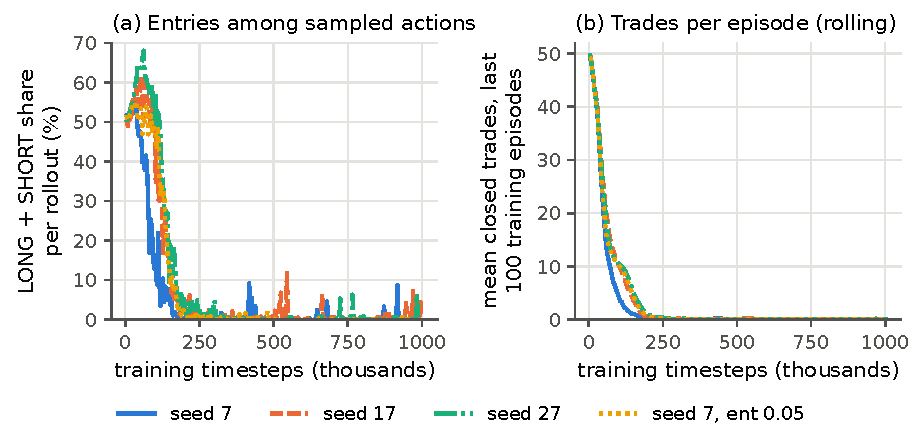
\includegraphics{figures/fig_training_collapse.pdf}
\caption{Attempt 1 training. (a) Share of LONG and SHORT among the 4,096 actions sampled in
each rollout. (b) Mean closed trades per episode over the last 100 completed training
episodes (a rolling window of about seven rollouts), recorded at the end of each rollout.
All four candidates nearly stopped sampling entries within the first quarter of training,
including the retry with five times the entropy coefficient.}
\label{fig:collapse}
\end{figure}

All four candidates followed the same path (Figure~\ref{fig:collapse}). The initial policy
sampled the four actions about equally and closed about 49 trades per 300-step episode,
losing about \$2.89 per episode, of which \$2.78 was fees. The share of LONG and SHORT among
sampled actions first fell below 1\% of a rollout at 176k, 209k, 229k and 184k steps for
seeds 7, 17 and 27 and the retry. In the last tenth of training episodes 97\% to 99\% had no
trade at all, and in the final rollout of every candidate LONG and SHORT were never
sampled; the actions were split between HOLD and EXIT (2,513 and 1,583 for seed 7). Mean
episode P\&L was negative in every tenth of training for every seed, and over the whole run
each candidate lost between \$368 and \$506, of which \$351 to \$488 was fees
(Appendix~\ref{app:diag}). The training callback recorded episode outcomes and action
counts but not the value loss, entropy, approximate KL divergence or explained variance,
so we cannot report those curves.

\subsection{Attempt 1: validation}\label{sec:val1}
\begin{table}[!htbp]
\centering
\caption{Attempt 1 on validation (25--28 September, 336,300 decisions, 284 seconds with
$|$gap$|\geq7$\bps). Fee 3.5\bps{} per side. Pre-fee P\&L is after spread, slippage and delay.}
\label{tab:val1}
\begin{tabular}{@{}lrrrrr@{}}
\toprule
Policy & Trades & Net P\&L (\$) & Pre-fee P\&L (\$) & Fees (\$) & Win rate \\
\midrule
PPO seed 7 (selected)        & 0 & 0.00 & 0.00 & 0.00 & -- \\
PPO seed 17                  & 0 & 0.00 & 0.00 & 0.00 & -- \\
PPO seed 27                  & 0 & 0.00 & 0.00 & 0.00 & -- \\
PPO seed 7, entropy 0.05     & 0 & 0.00 & 0.00 & 0.00 & -- \\
\midrule
Threshold 1\bps   & 11,895 & $-629.39$ & 69.62 & 699.01 & 2.1\% \\
Threshold 2\bps   &  6,708 & $-331.71$ & 62.92 & 394.64 & 3.8\% \\
Threshold 4\bps   &  2,014 &  $-83.17$ & 35.45 & 118.63 & 9.5\% \\
Threshold 7\bps   &    144 &   $-2.05$ &  6.43 &   8.48 & 34.0\% \\
Threshold 10\bps{} (selected) & 14 & 0.14 & 0.96 & 0.82 & 42.9\% \\
Threshold 20 and 100\bps & 0 & 0.00 & 0.00 & 0.00 & -- \\
Flat                         & 0 & 0.00 & 0.00 & 0.00 & -- \\
\bottomrule
\end{tabular}
\end{table}

All four PPO candidates made zero trades on validation (Table~\ref{tab:val1}). Their
deterministic actions differed: seed 7 chose HOLD in 99.3\% of decisions, while seeds 17
and 27 and the retry chose HOLD in 43.1\%, 36.6\% and 61.3\%. Nearly all their other
actions were EXIT while flat, which does nothing. Seed 17 and the retry issued 11 and 69
entry requests, all rejected by the freshness or end-of-episode checks. With every
candidate at zero trades and \$0, seed 7 was selected by the declared order.

\begin{figure}[!htbp]
\centering
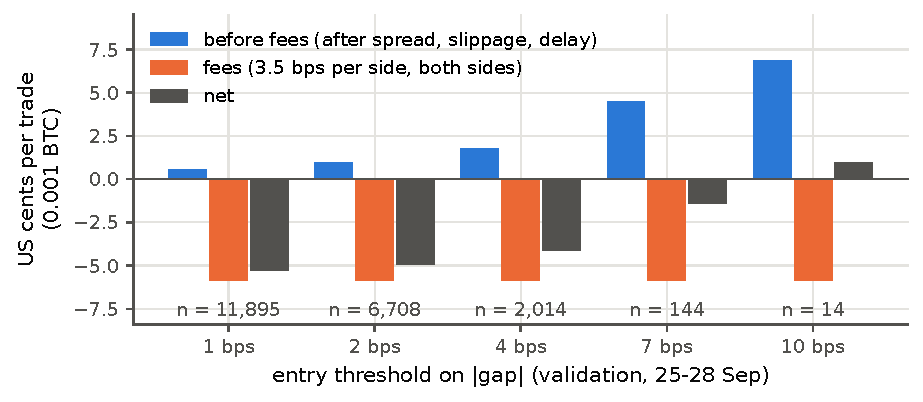
\includegraphics{figures/fig_edge_vs_fee.pdf}
\caption{Attempt 1 validation, threshold rules: mean P\&L per trade before fees, mean fee
per trade, and mean net P\&L per trade. $n$ is the number of trades. The gross gain per
trade grows with the threshold while the fee stays near 5.9 cents.}
\label{fig:edge}
\end{figure}

Net P\&L rose with the threshold up to 10\bps: low thresholds traded thousands of times and
lost heavily, and only the 10\bps{} rule finished positive, with \$0.14 over 14 trades.
Before fees, P\&L was positive at every threshold that traded, so the gap does predict the
direction of the next Hyperliquid move after spread, slippage and the 150\,ms delay. The
predicted move is small (Figure~\ref{fig:edge}): the mean pre-fee gain per trade was 0.59 US
cents at 1\bps{} and 6.86 cents at 10\bps, against a fee of about 5.9 cents per round trip.
Only at 10\bps{} did the average trade cover its fees.

\subsection{Attempt 1: held-out test}\label{sec:test1}
\begin{table}[!htbp]
\centering
\caption{Attempt 1 on the held-out test (29 September to 2 October, 1,140 episodes, 342,000
decisions, 331 seconds with $|$gap$|\geq7$\bps), run once after selection. Fee 3.5\bps{}
per side, 150\,ms delay.}
\label{tab:test1}
\begin{tabular}{@{}lrrrrrr@{}}
\toprule
Policy & Trades & Net P\&L (\$) & Fees (\$) & Win rate & Max DD (\$) & Selectivity \\
\midrule
PPO (seed 7)        & 0  & 0.00 & 0.00 & --    & 0.00 & 0.000 \\
Flat                & 0  & 0.00 & 0.00 & --    & 0.00 & 0.000 \\
Threshold 10\bps    & 16 & 1.19 & 0.95 & 87.5\% & 0.10 & 0.048 \\
\bottomrule
\end{tabular}
\end{table}

PPO made no trades on the test days (Table~\ref{tab:test1}). Its decision log has 338,980
HOLD and 3,020 EXIT-while-flat actions, no LONG or SHORT, and no entry requests, so its
\$0 is the flat control's result. The 10\bps{} threshold control made 16 trades (8 long,
8 short) for a net \$1.19, which is 0.012\% of the \$10,000 reference, after \$0.95 of fees.
It had 14 winning trades, a maximum drawdown of \$0.10 and a mean holding time of 10.5\,s;
12 exits came from the rule, 3 from the 30\,s limit and 1 from the episode end. Of its 41
entry requests, 25 were rejected by the freshness or timing checks. The result is small and
concentrated: 15 of the 16 trades and 98.7\% of the net P\&L fell on 30 September and
2 October, there was no trade on 1 October, and the three best trades produced 57\% of the
total.

This comparison depends on the fee. At 4.5\bps{} per side, the rate we later used for
attempt 2, every threshold that traded would have lost money on validation (the 10\bps{} rule
about \$0.10 over the same 14 trades, the 7\bps{} rule about \$4.47), so the declared
selection rule would have chosen the 100\bps{} threshold, which never trades. The test comparison would then have been \$0
against \$0. These figures re-price the recorded validation trades at the higher fee, which
is valid because the rule's trades do not change with the fee (Section~\ref{sec:sens1}); run
directly at 4.5\bps{} in attempt 2's evaluation, the same rule made 13 trades and lost \$0.08
(Table~\ref{tab:val2}). On the test days the 10\bps{} rule would still have made about
\$0.92 at 4.5\bps, but it would not have been selected.

\subsection{Attempt 1: cost sensitivity}\label{sec:sens1}
\begin{figure}[!htbp]
\centering
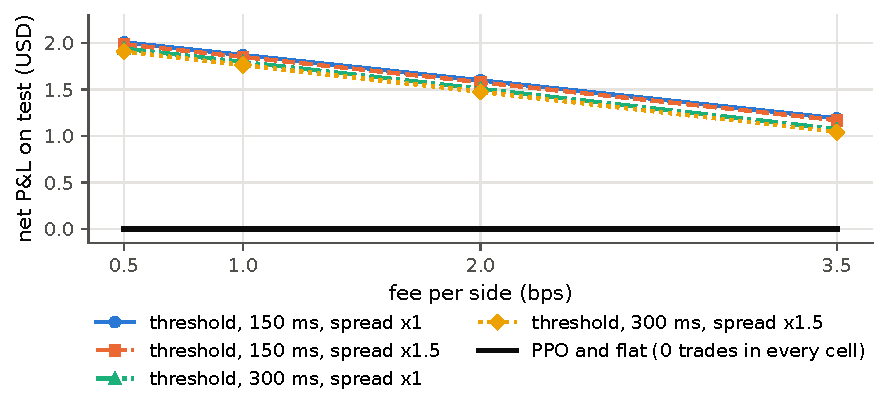
\includegraphics{figures/fig_sensitivity.pdf}
\caption{Attempt 1 test, net P\&L against fee per side for the 10\bps{} threshold control
under four delay and spread settings. The four lines nearly overlap; Table~\ref{tab:sensgrid}
in Appendix~\ref{app:sens} gives the exact values. PPO and flat made no trades in any of the
16 cells.}
\label{fig:sens}
\end{figure}

Across the 16 cost scenarios, PPO and flat made zero trades in every cell
(Figure~\ref{fig:sens}). The threshold control stayed positive in every cell, from \$2.01
(0.5\bps, 150\,ms, spread $\times1$) down to \$1.04 (3.5\bps, 300\,ms, spread $\times1.5$).
The 300\,ms delay changed its trade count from 16 to 17 and lowered its win rate at
3.5\bps{} from 87.5\% to 76.5\%. The sampled grid stops at 3.5\bps{} per side, so no
simulated cell brackets the fee at which the control breaks even. Because the rule's
decisions do not depend on the fee, its trades are the same at every fee level and its net
P\&L falls linearly with the fee rate. Solving for zero gives a break-even fee of 7.1 to
7.9\bps{} per side across the four delay and spread settings, an extrapolation from 16 or 17
trades.

\subsection{Attempt 2: opportunity-level PPO}\label{sec:att2}
The training split produced 317,232 candidates from 1,971 of the 5,984 training windows. Of
their counterfactual payoffs at 4.5\bps{} per side, 4,270 (1.35\%) were positive, 308,663
(97.30\%) negative and 4,299 zero (entries the environment rejected). The mean payoff was
$-7.66$ cents. The warm-start loss fell from about 0.32 to about 0.035 after two epochs
(0.035 to 0.036 across seeds) and to 0.025 after 50. PPO fine-tuning entered on 4 to 7 of
the 1,024 candidates in each seed's first rollout and on 111, 106 and 73 of 65,536 candidates
in total; seeds 17 and 27 entered on none in their last rollout. Training P\&L was
$-\$4.58$, $-\$5.31$ and $-\$4.17$ over 102, 99 and 66 trades.

\begin{table}[!htbp]
\centering
\caption{Attempt 2 on validation (25--28 September), fee 4.5\bps{} per side. Warm-start
checkpoints are supervised models before PPO fine-tuning.}
\label{tab:val2}
\begin{tabular}{@{}lrrl@{}}
\toprule
Candidate or control & Trades & Net P\&L (\$) & Note \\
\midrule
Seed 7 warm start (selected) & 0 & 0.000 & 1 entry, rejected \\
Seed 7 PPO                   & 0 & 0.000 & \\
Seed 17 warm start           & 4 & $-0.108$ & 1 winner \\
Seed 17 PPO                  & 0 & 0.000 & \\
Seed 27 warm start           & 4 & $-0.021$ & 2 winners \\
Seed 27 PPO                  & 0 & 0.000 & \\
\midrule
Threshold 6\bps           & 338 & $-15.102$ & \\
Threshold 7\bps           & 130 & $-3.965$ & \\
Threshold 9\bps           & 21 & $-0.302$ & \\
Threshold 10\bps          & 13 & $-0.079$ & \\
Threshold 12\bps          & 2 & 0.159 & best rule \\
Threshold 15\bps          & 1 & 0.142 & \\
Threshold 20\bps          & 0 & 0.000 & \\
Flat                      & 0 & 0.000 & \\
\bottomrule
\end{tabular}
\end{table}

On validation the four days offered about 755 candidates in 1,121 episodes, and 934 episodes
had none. All three PPO checkpoints and the seed-7 warm start made zero trades
(Table~\ref{tab:val2}). The seed-17 and seed-27 warm starts made four trades each and lost
money. The best threshold rule at 4.5\bps{} per side was 12\bps, with \$0.16 over 2 trades.
The selected candidate was the seed-7 warm start, chosen by tie-break among the zero-trade
candidates. It did not meet the fresh-test gate, so attempt 2 never opened 3 October. The
outcome file for this run records the result as a failure to learn profitable trading.

% ------------------------------------------------------------------ 6
\section{Why PPO learned not to trade}\label{sec:why}

We identify five properties of the problem and the training set-up that plausibly
contributed to the failure; we did not test them separately. We found no fault in the
environment or evaluation code: their tests pass, unscaled rewards reconcile with the trade
ledger, and the threshold control trades profitably in the same environment. The PPO
inference path (saved model, frozen normalisation and action decoding) is covered only by the
saved-model and normalisation equivalence tests.

\subsection{Staying flat returns zero, which random entry cannot beat}
With a round trip costing about 7.3\bps{} and a median absolute gap of 1.3\bps, almost every
entry has a negative expected value. The initial random policy lost \$2.89 per episode.
Starting from that policy, lowering the probability of entering raises the expected return,
and the flat policy's return of zero is higher than that of any policy that enters at random.
It is not the best policy available: the 10\bps{} rule beat it on validation and test. Once
entries became rare, few entry samples remained to update their probability; we did not log
advantages, so we cannot confirm this mechanism. Figure~\ref{fig:collapse} shows entries
becoming rare within the first quarter of training for every seed.

\subsection{Trades that cover their costs are rare}\label{sec:rare}
On validation, 284 of 336,300 decision seconds (0.084\%) had an absolute gap of 7\bps{} or
more and 31 had 10\bps{} or more. The average threshold trade covered its fees only at
10\bps, where 14 trades in four days netted about 1 cent each (Figure~\ref{fig:edge}). To
learn to enter at those seconds and nowhere else, the agent must pick out that gain from a
reward stream in which a wrongly timed entry costs about 6 cents.

Large gaps often coincide with stale Hyperliquid quotes. On the test days the quote age or
receive age exceeded 1,000\,ms in 2.5\% of all decision seconds, but in 31\% of seconds with
an absolute gap of 7\bps{} or more and in 49\% of those with 10\bps{} or more (on validation,
1.7\%, 21\% and 39\%). The entry-freshness rule refuses entries at exactly those seconds;
with the timing check, it rejected 25 of the threshold control's 41 test entry requests. Part
of the measured gap is therefore likely the age of the Hyperliquid snapshot rather than a
tradable price difference. The rule is also applied to ages that include clock offset
(Section~\ref{sec:asym}).

\begin{figure}[!htbp]
\centering
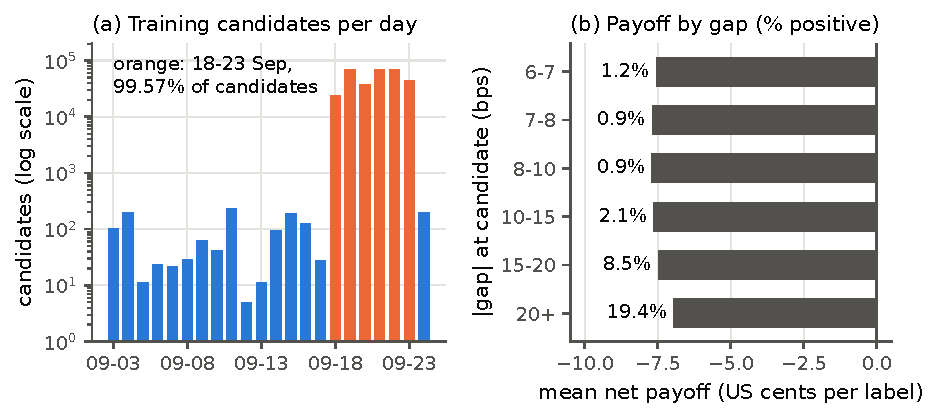
\includegraphics{figures/fig_attempt2_labels.pdf}
\caption{Attempt 2 training labels at 4.5\bps{} per side. (a) Candidates per training day on
a log scale; the six orange days (18--23 September) hold 99.57\% of them. (b) Mean
counterfactual net payoff by absolute gap at the candidate, with the share of positive
labels printed beside each bar. The mean is negative in every bucket.}
\label{fig:labels}
\end{figure}

Attempt 2's training labels were also negative on average in every gap bucket, including
gaps of 20\bps{} or more, where 19.4\% were positive (Figure~\ref{fig:labels}b and
Appendix~\ref{app:labels}). But 99.57\% of them came from the six basis days
(Section~\ref{sec:regime}), so they say little about the other days.

\subsection{Attempt 1 had two ways of doing nothing}
While the agent is flat, EXIT has the same effect as HOLD. In the final training rollouts
the sampled actions were split between the two, and three of the four deterministic
validation policies chose EXIT in 39\% to 63\% of decisions. A policy split evenly between
HOLD and EXIT keeps half of the maximum entropy ($\ln 2$ of $\ln 4$ nats) without entering.
The retry with five times the entropy coefficient nearly stopped entering at about the same
point as the original seed 7 (184k against 176k steps) and made no validation trades. We
read this as evidence that the redundant action made abstention easier to reach in
attempt 1. Attempt 2 had a single way to abstain (skip), and its PPO seeds also made zero
validation trades, so the redundant action is at most a contributing factor and was not
required for abstention. We did not run an ablation that removes it from attempt 1.

\subsection{The training period was dominated by a basis regime}\label{sec:regime}
Of the training seconds with an absolute gap of 7\bps{} or more, 99.7\% fell on
18--23 September, and so did 99.57\% of attempt 2's candidates (Figure~\ref{fig:labels}a).
Only 17 of those 315,861 candidates had a positive signed gap. On the six basis days 99.72\%
of the counterfactual trades ran 30\,s or more from decision to completion, nearly all
exactly 31\,s, which is how a close at the 30\,s holding limit shows in the replay; on the
other 16 training days the share was 27.0\% (median 8\,s). Only 1.27\% of the labels on the
six days were positive (mean $-7.69$ cents), against 19.9\% on the other 16 days, where the
mean label was still $-1.81$ cents. In attempt 1 these six days supplied 1,623 of the 5,984
training windows (27.1\%); in attempt 2 about 99.5\% of PPO decisions came from them. In
attempt 2 the labels on these days show that large gaps rarely closed within 30\,s; we did
not test whether attempt 1 learned this.

Offsets were not confined to the training period. The first validation day, 25 September,
had a daily median gap of $-2.8$\bps, larger in size than on 18 September ($-2.4$\bps),
although only 0.25\% of its seconds reached 7\bps{} against 22\% on 18 September. After we
subtracted each window's mean gap, 83 validation seconds and 127 test seconds still deviated
by 7\bps{} or more, against 284 and 331 before; on the 16 non-basis training days the count
fell only from 890 to 643. Slow offsets therefore produced most of the large gaps on
validation and test as well.

\subsection{The warm start learned to skip because almost all training labels lost money}
Skip was the loss-minimising answer on these labels: 97.3\% were negative, and positives
were 1.35\% of the examples but carried 0.51\% of the weight under the $|$payoff$|$
weighting. The labels also overlap in time. Most are consecutive seconds within the same
windows of the same six days, and their counterfactual trades could not all be taken, so the
effective number of independent examples is far below 317,232. The weighted loss fell from
about 0.32 to about 0.035 within two epochs and moved little after that. PPO then started from
a policy that almost never entered, and entries made up only 0.11\% to 0.17\% of its
decisions.

\subsection{What the threshold control does and does not show}\label{sec:control}
The \$1.19 on the test belongs to the fixed 10\bps{} rule, not to PPO. It shows that the
environment allows trades that cover their costs at 3.5\bps{} per side and that the rule
found 16 of them on the test days. It does not show a dependable edge: the profit rests on
16 trades concentrated on two days, and the rule was selected only because validation was
priced at 3.5\bps{} (Section~\ref{sec:test1}).

% ------------------------------------------------------------------ 7
\section{Responsible AI}\label{sec:rai}

\subsection{Fairness}
Latency arbitrage earns money by trading against quotes that have not caught up with the
market. The other side of those trades is the liquidity provider whose quote is stale, often
a slower participant. Budish et al.~\cite{budish} argue that this race is a cost to
liquidity providers that is passed on to all traders as wider spreads. A working version of
our agent would be on the fast side of that transfer. Our results suggest that, after taker
fees, the amount available to a small taker on this pair is small, but the concern applies
to any team with lower fees or faster infrastructure. Nothing in this project connects to a
live market or uses capital.

\subsection{Transparency}
The experiment protocols were written and hashed before training, every prepared episode and
model file has a SHA-256 hash, and the test runs logged every decision, fill and trade.
Failed experiments were kept. The two PPO runs each have an outcome file that records the
failure and states that no success claim is permitted; the diagnostic in
Appendix~\ref{app:value} has only a status file, whose conclusion calls its single fresh-day
trade net positive. Each table and figure in this report names the split it comes from, and
the statistics we computed for this report beyond the saved run summaries are reproduced by a
script stored with it (Appendix~\ref{app:repro}).

\subsection{Accountability}
Policies were selected on validation data only, and the test was run once, after the
selection file was frozen. The test days are now recorded as spent. Risk limits are enforced
by the environment rather than left to the learned policy. The AI-use statement below
records which parts were produced by AI agents, and the team members are responsible for
reviewing them.

\subsection{Trust and calibrated claims}
The main risk of misuse of these results is over-reading them: describing a zero-trade
policy as one that ``avoided losses'', or describing the threshold control's profit as a
reinforcement learning result (Section~\ref{sec:control}). We report zero trades as
abstention and give the trade count next to every P\&L figure, so that results resting on a
handful of trades are visible as such.

% ------------------------------------------------------------------ 8
\section{Limitations and threats to validity}\label{sec:limits}

\subsection{Funding is assumed zero}\label{sec:funding}
The source table has no funding rates, so funding is set to zero in every result. Positions
last at most 30\,s, so the direct effect on single trades is probably small, but we could not
check it, and a funding difference between the venues is one possible cause of the
18--23 September basis.

\subsection{Quality-filtered subset}\label{sec:subset}
We kept 95.43\% of the five-minute windows. Dropping windows with stale Hyperliquid quotes
removes some of the moments when the slower venue lags most, which may bias the data toward
calmer periods. Keeping only windows in which every row passed the quality checks also
conditions each episode on the absence of a feed outage later in the same five minutes,
which a live trader would not know. One window per day is dropped for a preparation reason
unrelated to quality (Section~\ref{sec:align}).

\subsection{Sampled books}
Both feeds are snapshot streams, and Hyperliquid's has 5 levels and about 1.84 updates per
second. Between snapshots the true book is unknown, and a fill at +150\,ms uses the latest
recorded Hyperliquid snapshot, which can be close to a second old. The quote age we report
includes a median of about 270\,ms since the snapshot was received, and the rest mixes
network delay with clock offset between machines.

\subsection{No market impact or competition}
Orders take displayed liquidity without moving later prices, and other traders who react to
the same Binance move are not modelled. The delay is fixed at 150\,ms (300\,ms in stress
tests) rather than drawn from a measured distribution.

\subsection{Small trade counts}\label{sec:counts}
The threshold control made 14 trades on validation and 16 on test, and the attempt-2
candidates made between 0 and 4. These counts are too small to estimate a profit rate with
useful precision.

\subsection{Reuse of evaluation data}
The test days of attempt 1 have been seen and cannot serve as fresh evidence. Attempt 2 was
designed after attempt 1 failed and was selected on the same validation days, and the fee
setting moved from 3.5 to 4.5\bps{} between attempts. The fresh day of 3 October was later
opened by a non-RL diagnostic (Appendix~\ref{app:value}), so no untouched day remains in the
current dataset.

\subsection{Instrument identity and the basis}\label{sec:identity}
The rows carry no symbol field. The Binance stream name \texttt{btcusdt@depth20@100ms} does
not by itself record whether the spot or the futures endpoint was used, and the two venues
may quote Bitcoin against different stablecoins. A quote-currency difference, a premium or
funding difference between the venues, or a venue-specific event could each explain the
18--23 September basis; we did not verify any of them.

\subsection{Limited search}\label{sec:search}
Each attempt used one hyperparameter configuration (plus the one entropy retry in attempt 1)
and a fixed training budget. We did not try reward shaping, an action set without the
redundant EXIT, a value-based agent such as DQN~\cite{dqn}, which the proposal listed as an
optional comparison, or a longer training run. The observation includes the absolute
Hyperliquid price, which drifts over time and relies on the training-set normalisation.
Optimisation diagnostics (value loss, entropy, KL divergence) were not logged. The study
covers one pair of venues for one month.

% ------------------------------------------------------------------ 9
\section{Conclusion}\label{sec:conclusion}

We built a causal replay of 30 days of Binance and Hyperliquid order books, a cost-aware
environment with delayed fills against the recorded book, and two pre-declared PPO
experiments with validation-only selection. Neither PPO design learned to trade. The
four-action agent cut its share of entry actions below 1\% within about 230,000 of its
1,000,000 training steps on every seed, made zero trades on validation, and made zero trades
on the held-out test, where a fixed 10\bps{} threshold rule made \$1.19 over 16 trades at
3.5\bps{} per side. At 4.5\bps{} per side the declared selection rule would not have chosen
that rule. The opportunity-level agent with a supervised warm start also made zero
validation trades on all three PPO seeds. The project did not reach its stated goal of
beating the fixed rule under identical costs. Under these costs staying flat returned zero
while random entry lost money, cost-covering trades were rare, and the training period's
large gaps came mostly from a six-day basis that did not close within the holding limit.
Attempt 1's redundant EXIT action may have made abstention easier to reach, but attempt 2
abstained without it.

\subsection*{Lessons and next steps}
We changed the set-up once (attempt 2) and the algorithm not at all, so we cannot say which
matters more. Next steps for both:
\begin{itemize}
\item Attempt 2 removed the redundant action, among other changes, and still abstained, so
changing the action set is not enough on its own.
\item Separate large gaps that come from a slow offset between venues from gaps that come
from one venue lagging, for example by measuring the gap relative to a slowly moving
estimate of the basis. Offsets produced most large gaps on all three splits, not only in
training.
\item Merge labels from consecutive seconds of the same gap event into one opportunity.
\item Keep reporting the flat and threshold controls next to the agent, report results at
more than one fee, require more trades before any claim of profit, and use newly recorded
days for the next test, since every day in the current dataset has now been examined.
\item Log PPO's optimisation statistics (value loss, entropy, KL divergence and advantages)
so that a collapse can be diagnosed while it happens, and try the untested options in
Section~\ref{sec:search}, such as a value-based agent or a broader hyperparameter search.
\end{itemize}

% ------------------------------------------------------------------ roles
\section*{Team roles}
\addcontentsline{toc}{section}{Team roles}
Roles to be confirmed by each member. The proposal planned the following division; the
AI-use statement below records which parts AI agents implemented.
\begin{itemize}
\item \emph{Kerk Tai Heng}: data preparation and episode generation.
\item \emph{Member 2}: replay environment and transaction-cost model.
\item \emph{Member 3}: baseline strategy and evaluation tools.
\item \emph{Member 4}: PPO training and tuning.
\item \emph{Member 5}: held-out evaluation and fee sensitivity tests.
\item \emph{Member 6}: Responsible-AI analysis, report integration and presentation.
\end{itemize}
\todo{Replace the placeholders and edit each line so that it states what each member actually
did. Adjustments from the proposal are allowed but should be stated.}

% ------------------------------------------------------------------ AI use
\section*{AI-use statement}
\addcontentsline{toc}{section}{AI-use statement}
AI coding agents did a large share of the engineering and writing in this project, under the
team's direction. An OpenAI Codex-based coding agent implemented substantial parts of the
pipeline: the data preparation and quality checks, the replay environment and cost model, the
threshold and flat controls, the evaluation code, the PPO training and experiment drivers for
both attempts, the gradient-boosting diagnostic in Appendix~\ref{app:value}, and the run-report
scripts. Anthropic's Claude audited the saved run artifacts against the source code,
recomputed the statistics marked as derived in this report, wrote the figure script
(\texttt{make\_figures.py}), and drafted the text of this report. The research question, the
data recording, the cost assumptions and the evaluation plan come from the team's proposal.
The team reviewed the agents' output and is responsible for the code, the results and this
report. ChatGPT was used to edit the proposal for clarity.

\todo{Confirm or edit this statement so that it matches exactly what each member and each AI
tool did, including which parts of the code and text the team wrote or rewrote, before
submission.}

\phantomsection\label{bodyend}
% ------------------------------------------------------------------ references
\clearpage
\begin{thebibliography}{99}
\bibitem{budish} Budish E, Cramton P, Shim J. The high-frequency trading arms race: frequent
batch auctions as a market design response. Q J Econ. 2015;130(4):1547--621.
\bibitem{report} Cross-venue latency arbitrage feasibility study: Binance--Hyperliquid BTC
perpetuals. Internal report supplied to the project team; 2026. Unpublished.
\bibitem{ppo} Schulman J, Wolski F, Dhariwal P, Radford A, Klimov O. Proximal policy
optimization algorithms [Preprint]. arXiv:1707.06347. 2017 [cited 2026 Oct 5]. Available
from: \url{https://arxiv.org/abs/1707.06347}
\bibitem{nevmyvaka} Nevmyvaka Y, Feng Y, Kearns M. Reinforcement learning for optimized trade
execution. In: Proceedings of the 23rd International Conference on Machine Learning; 2006
Jun 25--29; Pittsburgh, PA. New York: ACM; 2006. p. 673--80.
\bibitem{guide} Data and training guide: Binance--Hyperliquid order-book data set. Internal
project document; 2026 Oct 4. Unpublished.
\bibitem{gym} Towers M, Kwiatkowski A, Terry J, Balis JU, De Cola G, Deleu T, et al.
Gymnasium: a standard interface for reinforcement learning environments [Preprint].
arXiv:2407.17032. 2024 [cited 2026 Oct 5]. Available from:
\url{https://arxiv.org/abs/2407.17032}
\bibitem{sb3} Raffin A, Hill A, Gleave A, Kanervisto A, Ernestus M, Dormann N.
Stable-Baselines3: reliable reinforcement learning implementations. J Mach Learn Res.
2021;22(268):1--8.
\bibitem{gae} Schulman J, Moritz P, Levine S, Jordan MI, Abbeel P. High-dimensional
continuous control using generalized advantage estimation [Preprint]. arXiv:1506.02438.
2015 [cited 2026 Oct 5]. Available from: \url{https://arxiv.org/abs/1506.02438}
\bibitem{henderson} Henderson P, Islam R, Bachman P, Pineau J, Precup D, Meger D. Deep
reinforcement learning that matters. In: Proceedings of the Thirty-Second AAAI Conference on
Artificial Intelligence; 2018 Feb 2--7; New Orleans, LA. Palo Alto (CA): AAAI Press; 2018.
p. 3207--14.
\bibitem{dqn} Mnih V, Kavukcuoglu K, Silver D, Rusu AA, Veness J, Bellemare MG, et al.
Human-level control through deep reinforcement learning. Nature. 2015;518(7540):529--33.
\bibitem{sklearn} Pedregosa F, Varoquaux G, Gramfort A, Michel V, Thirion B, Grisel O, et al.
Scikit-learn: machine learning in Python. J Mach Learn Res. 2011;12:2825--30.
\end{thebibliography}

% ------------------------------------------------------------------ appendices
\clearpage
\appendix
\renewcommand{\thesection}{\Alph{section}}
\begin{center}{\Large\bfseries Appendices}\end{center}

\section{Reproducibility and provenance}\label{app:repro}
All runs used Python 3.12.3, NumPy 2.5.3, PyTorch 2.14.1 (CPU), Gymnasium 1.3.0 and
Stable-Baselines3 2.9.0; the diagnostic in Appendix~\ref{app:value} also used scikit-learn
1.9.1~\cite{sklearn}. Training ran on a CPU: about 65 minutes for the four attempt-1
candidates and about 24 minutes for the whole attempt-2 pipeline. The saved artifacts are:
\begin{itemize}
\item Prepared data: the 30-day set in \texttt{data/recorded-30d/}, whose manifest has
SHA-256 \texttt{afa9c485\ldots46b1}, and the 3 October holdout in
\texttt{data/recorded-fresh-2026-10-03/}.
\item Attempt 1: \texttt{runs/recorded-ppo-2026-10-04/} (git commit \texttt{98cbef6},
protocol SHA-256 \texttt{84d1e980\ldots6f40}, selection SHA-256
\texttt{c23f9219\ldots9f07}).
\item Attempt 2: \texttt{runs/opportunity-ppo-2026-10-04/}; an independent audit before
selection confirmed that source and manifest hashes matched and that no fresh-day output
existed.
\item Appendix~\ref{app:value} diagnostic: \texttt{runs/opportunity-value-2026-10-04/}.
\end{itemize}
The figures and the statistics this report computed beyond the saved run summaries are
produced by \texttt{docs/report\_v1/make\_figures.py}, which reads only saved artifacts and
writes \texttt{docs/report\_v1/generated/derived\_stats.json}. They are the daily gap
statistics, per-decile training statistics, per-trade threshold economics, the threshold
rules re-priced at 4.5\bps{} per side, the attempt-2 label statistics, and, per split, the
Hyperliquid quote and receive ages, spreads, prices, snapshot rates and stale-quote shares.
While checking the artifacts we found three discrepancies in older project documents: the
data guide's update rates (8.24 and 1.63 per second) do not match its own rows per day, the
proposal's ``roughly 26 million time-aligned, ten-level order-book snapshots'' does not
match the 28.9 million raw rows with five Hyperliquid levels, and the 3 October data
manifest still says no trading evaluation was performed on that day although the run in
Appendix~\ref{app:value} later evaluated it.

\section{PPO hyperparameters}\label{app:hyper}
\begin{table}[H]
\centering
\caption{PPO settings for both attempts. Attempt-2 values for clip range, $\lambda$, value
coefficient and gradient clip are the library defaults and were recorded with the run. An
attempt-2 training step is one candidate decision.}
\label{tab:hyper}
\begin{tabular}{@{}lrr@{}}
\toprule
Setting & Attempt 1 & Attempt 2 \\
\midrule
Action space & HOLD, LONG, SHORT, EXIT & skip, enter \\
Observation features & 17 & 18 \\
Training steps & 1,003,520 & 65,536 \\
Steps per rollout & 4,096 & 1,024 \\
Minibatch size & 256 & 128 \\
Epochs per rollout & 5 & 5 \\
Learning rate & $3\times10^{-4}$ & $10^{-4}$ \\
Discount $\gamma$ & 0.999 & 1.0 \\
GAE $\lambda$ & 0.95 & 0.95 \\
Clip range & 0.2 & 0.2 \\
Entropy coefficient & 0.01 (retry 0.05) & 0.005 \\
Value coefficient & 0.5 & 0.5 \\
Gradient-norm clip & 0.5 & 0.5 \\
Hidden layers (policy and value) & 64, 64 & 32, 32 \\
Observation clip & 10 & 10 \\
Reward scale in training & 100 & 100 \\
Seeds & 7, 17, 27 (+ retry 7) & 7, 17, 27 \\
Warm start & none & 50 epochs \\
\bottomrule
\end{tabular}
\end{table}

\section{Attempt 1 training diagnostics per candidate}\label{app:diag}
\begin{table}[H]
\centering
\caption{Attempt 1 training, from the per-episode monitor logs (3,345 training episodes per
candidate). ``First decile'' and ``last decile'' are the first and last tenth of training
episodes. ``Entry share below 1\%'' is the training step at the end of the first rollout in
which LONG and SHORT made up less than 1\% of sampled actions. ``Retry'' is seed 7 with
entropy coefficient 0.05.}
\label{tab:diag}
\begin{tabular}{@{}lrrrr@{}}
\toprule
 & Seed 7 & Seed 17 & Seed 27 & Retry \\
\midrule
Training time (s) & 1,017 & 984 & 896 & 978 \\
Total trades & 6,262 & 8,568 & 8,742 & 8,100 \\
Total net P\&L (\$) & $-368.24$ & $-495.97$ & $-506.13$ & $-472.74$ \\
Total fees (\$) & 351.32 & 476.75 & 487.78 & 453.77 \\
Episodes with no trade & 84.5\% & 79.4\% & 78.5\% & 79.4\% \\
Trades per episode, first decile & 17.47 & 22.08 & 21.44 & 20.38 \\
Trades per episode, last decile & 0.066 & 0.105 & 0.042 & 0.006 \\
No-trade episodes, last decile & 99.1\% & 97.0\% & 98.2\% & 99.4\% \\
Final rollout HOLD & 2,513 & 2,055 & 2,021 & 2,375 \\
Final rollout EXIT & 1,583 & 2,041 & 2,075 & 1,721 \\
Entry share below 1\% at step & 176,128 & 208,896 & 229,376 & 184,320 \\
Validation HOLD share & 99.3\% & 43.1\% & 36.6\% & 61.3\% \\
Validation entry requests & 0 & 11 & 0 & 69 \\
\bottomrule
\end{tabular}
\end{table}
Training rollouts sample from the stochastic policy, while validation and test use the most
likely action. This is why a few training episodes late in training still contain trades
while the deterministic policies never trade.

\section{Attempt 1 full test sensitivity grid}\label{app:sens}
\begin{table}[H]
\centering
\caption{Threshold control (10\bps) on the test days under each cost scenario. PPO and flat
made 0 trades and \$0 in all 16 scenarios. Break-even is the fee per side at which net P\&L
reaches zero, computed from the fixed trade set (not simulated).}
\label{tab:sensgrid}
\begin{tabular}{@{}rrrrrrr@{}}
\toprule
Delay (ms) & Spread & Fee 0.5 & Fee 1.0 & Fee 2.0 & Fee 3.5 & Break-even \\
 & mult. & (\$) & (\$) & (\$) & (\$) & (bps/side) \\
\midrule
150 & 1.0 & 2.005 & 1.869 & 1.597 & 1.188 & 7.86 \\
150 & 1.5 & 1.985 & 1.848 & 1.576 & 1.168 & 7.79 \\
300 & 1.0 & 1.939 & 1.794 & 1.506 & 1.072 & 7.21 \\
300 & 1.5 & 1.906 & 1.762 & 1.473 & 1.040 & 7.10 \\
\bottomrule
\end{tabular}
\end{table}
Trades were 16 at 150\,ms and 17 at 300\,ms in every fee setting. Win rates at 3.5\bps{} were
87.5\% (150\,ms) and 76.5\% (300\,ms); at 0.5\bps{} every trade won.

\section{Data-quality detail}\label{app:quality}
\begin{table}[H]
\centering
\caption{Grid rows (of 7,776,000) that failed a quality rule, 3 September to 2 October.
A failed row rejects its whole five-minute window.}
\label{tab:quality}
\begin{tabular}{@{}lrr@{}}
\toprule
Reason & Binance & Hyperliquid \\
\midrule
Receive age over 2,000\,ms & 176 & 3,180 \\
Quote age over 3,000\,ms & 166 & 3,065 \\
No earlier snapshot & 30 & 103 \\
Latest snapshot invalid & 0 & 0 \\
\midrule
Gap over 250\bps{} (either venue) & \multicolumn{2}{c}{0} \\
Receive gaps over 2\,s (count) & 9 & 504 \\
Longest receive gap & 31.7\,s (21 Sep) & 173.0\,s (26 Sep) \\
\bottomrule
\end{tabular}
\end{table}
Rejected windows per day were 9 to 21 on the 22 training days (most on 15 September); 18, 10,
1 and 2 on the validation days; and 4, 2, 3 and 3 on the test days. Of the 504 Hyperliquid
receive gaps, 455 were in the training period, 35 in validation and 14 in test. On 3 October
286 of 288 windows were kept and Hyperliquid had 3 gaps over 2\,s (longest 109.4\,s). Every
episode file holds 900 rows with the fields listed in the data schema, and in all 8,531
episodes the decision rows are rows 0, 3, 6, \ldots{} and fall on whole seconds.

\section{Attempt 2 label statistics}\label{app:labels}
\begin{table}[H]
\centering
\caption{Attempt 2 counterfactual labels by absolute gap at the candidate (training split,
4.5\bps{} per side). Payoffs are in US cents for 0.001\,BTC.}
\label{tab:labels}
\begin{tabular}{@{}lrrr@{}}
\toprule
$|$gap$|$ (bps) & Candidates & Positive share & Mean net payoff (cents) \\
\midrule
6--7    & 32,879  & 1.2\%  & $-7.56$ \\
7--8    & 50,466  & 0.9\%  & $-7.69$ \\
8--10   & 141,738 & 0.9\%  & $-7.70$ \\
10--15  & 89,218  & 2.1\%  & $-7.64$ \\
15--20  & 2,281   & 8.5\%  & $-7.49$ \\
20 or more & 650  & 19.4\% & $-6.95$ \\
\midrule
All     & 317,232 & 1.35\% & $-7.66$ \\
\bottomrule
\end{tabular}
\end{table}
The median payoff was $-7.59$ cents; positive labels averaged $+2.94$ cents and negative
labels $-7.92$ cents, and the mean fee per traded label was 7.53 cents. On the six basis days
1.27\% of labels were positive (mean $-7.69$ cents); on the other 16 training days, 1,371
candidates in all, 19.9\% were positive (mean $-1.81$ cents). PPO fine-tuning lost \$4.58,
\$5.31 and \$4.17 on training replay (seeds 7, 17, 27), paying \$7.54, \$7.32 and \$4.96 in fees.

\section{Non-RL diagnostic: expected-value selector (not PPO)}\label{app:value}
After attempt 2, the coding agent ran a supervised diagnostic that is not reinforcement
learning and is not part of the PPO results. Two gradient-boosted regression models
(scikit-learn \texttt{HistGradientBoostingRegressor}, 200 iterations) were fitted to predict
the counterfactual net payoff of the 317,232 attempt-2 training candidates. Each model was
paired with a minimum predicted value of \$0 or \$0.01 for entering, giving four candidates;
the six attempt-2 checkpoints were re-evaluated unchanged alongside them. Validation used
3.5\bps{} per side, so the fee changed again. The regressors were fitted to payoffs labelled
at 4.5\bps{} per side. During replay at 3.5\bps{} the cost-excess input was lowered by 2\bps{}
to match its training value, so the entry rule compared a payoff predicted at 4.5\bps{} per
side with the margin. The gate for opening 3 October required only positive validation net
P\&L with at least one trade; it did not require beating the threshold rule.

On validation the selected model (15 leaves, minimum 50 samples per leaf, \$0 margin) made
\$0.058 over 2 trades, while the 12\bps{} threshold rule made \$0.193 over 2 trades and the
10\bps{} rule \$0.139 over 13. All three PPO checkpoints again made zero trades. The selected
model passed the gate, so 3 October was opened. That day offered only 4 candidates in 286
episodes. The model and the 12\bps{} threshold rule skipped the same three and took the same
one, a 14.4\bps{} gap at 21:05:18 UTC: a short of 0.001\,BTC held for 5\,s that netted
\$0.045 at 3.5\bps{} per side and \$0.028 at 4.5\bps. The two policies' decision, trade and
fill logs are byte-identical. One trade identical to the threshold rule's is no evidence of
a learned edge, and running this diagnostic used up the last untouched day of data.

\end{document}
